\documentclass{beamer} 

% Michael Maier, 2014.
% CC-BY-SA 3.0 at

\usepackage[utf8]{inputenc}
\usepackage[ngerman]{babel}

\title{OpenStreetMap - Die freie Weltkarte nutzen} 
\author{Michael Maier \textless Michael.Maier@student.tugraz.at\textgreater} 
\date{13. Jänner 2014} 

\usetheme{Antibes}

\hypersetup{colorlinks=true,urlcolor=blue,linkcolor=white}

%\usebackgroundtemplatei{
%
\includegraphics[width=\paperwidth,
%height=0.8\paperheight]{mag_map.png}
%}

\begin{document}

%\maketitle

\begin{frame} 


\begin{figure}
  \centering
  
\includegraphics[width=.5\textwidth]{mag_map.png}
\end{figure}

\begin{center}
\Huge{OpenStreetMap\\}
\end{center}

\begin{center}
\Large{\emph{Die freie Weltkarte nutzen}}
\end{center}

\end{frame}


% Zielgruppe
% * Google, Konkurrenten
% * Landes-GISler
% * Firmen

% Wichtig:
% Quality Assurance
% * Es gibt automatische Q/A-Tools
% * kaum Streitfälle - wenn dann Mailinglist, Data Working Group
% * 
% tolle Bilder herzeigen!
% * irgendein Zoo
% * 3D
% * Tolle Kartenstile:
%     * OSM-Fr?
%     * stamen watercolor
%     * pistemap
%     * bicycle map
%     * OpenSeaMap
%
% Dokumentation (nenne es doku und nicht Wiki → verwirrent)
% wenn wo doku fehlt, selber mitschreiben?

% Vorteile
% * aktuell!
%   wenn nicht aktuell: OSM Verbessern!
%  - JEDE Karte ist in dem Moment veraltet, wo sie gedruckt wurde...
%  - impressive Number: changesets/day - oder sekunde/minute 
% changeset 19980639 an  13 Jan 2014 22:59:23
% 16561091 an 15 Jun 2013 11:10:25
% = 3419548 in 208d = 16500/d = 685/h = 12/Minute
% oder 2M nodes/day dazu
%
% * 100e verschiedene Kartenstile 
%   den eigenen leichtgemacht mit Tilemill
% * Datenversionierung!
% * Language-Independent
%   show http://toolserver.org/~osm/locale/ru.html
% * jetzt in 3D!
% switch2osm net vergessen!
% HOT Team nicht vergessen!

% Dienst: Geocoder!
% Dienste: Routing!

% * kurze OSM-Vorstellung, Geschichtliches, Motivation
% * Technogie, Datenmodell, Lizenz
% * OSM Nutzen: Rohdaten, Web-Dienste, Apps

\begin{frame}{Vorstellung}

  \begin{itemize}
    \item Michael Maier \textless \href{mailto:Michael.Maier@student.tugraz.at}{Michael.Maier@student.tugraz.at}\textgreater
    \item Student an der TU Graz (Telematik)
    \item OpenStreetMap als Hobby seit Juli 2010
    \item Leite den Grazer OSM-Stammtisch seit Mai 2011
    \item Vorträge und Workshops zum Thema OSM seit 2012
    \item Freiberuflich OSM-Aufträge und Consulting
%    \begin{itemize}
%      \item OSM-username: \emph{\href{http://www.openstreetmap.org/user/species}{species}}
%      \item Mapping-area Graz, Leoben on bicycle, motorbike or on public transport
%    \end{itemize}
  \end{itemize}
\end{frame}

\section{Einleitung}


% Folien zu
% * kurze OSM-Vorstellung, Geschichtliches, Motivation
%  1. OSM-Vorstellung
  % was ist es
  % wer steckt dahinter?
% Geschichtliches
  % Gegründet ... steve
  % user-wachstum
% Motivation
  % gegründet, weil es keine freien Geodaten gab
  % Wunschtraum: eine DB weltweit

\begin{frame}{Was ist OpenStreetMap}

\begin{itemize}
  \item OpenStreetMap (OSM) ist eine freie Weltkarte nach dem Wiki-Prinzip "`Wikipedia der Karten"'
    \begin{itemize}
      \item \emph{Eigentlich eine Geo-Datenbank}
    \end{itemize}
\pause
  \item Entsteht aus der Arbeit von \textgreater 1,4\,M Hobbykartografen "`\emph{Mapper}"'

 \item Das komplette "`planet file"' ist ca. 427\,GB groß (xml) (Dienstag):
  \begin{itemize}
    \item 2.161.810.973 Nodes
    \item 213.302.643 Ways
    \item 2.326.786 Relations
  \end{itemize}

\end{itemize}


% \begin{center}
% \includegraphics[width=5.5cm]{sotm.jpg}
% \end{center}

\end{frame}

\begin{frame}{Wer steht hinter OpenStreetMap}

  \begin{itemize}
    \item OpenStreetMap Foundation (Server, Rechtliche Vertretung)
      \pause
    \item Mapper ($\sim$30.000 aktiv), meist ohne Geo-Hintergrund
    \begin{itemize}
      \item Jährliche Konferenz - "`State of the Map"', heuer: Buenos Aires
    \end{itemize}
      \pause
    \item Universitäten
    \begin{itemize}
      \item Bakk-, Master- und Doktorarbeiten mit OSM
      \item Server-Hosting
    \end{itemize}
      \pause
    \item Organisationen, die Daten sponsern
    \begin{itemize}
      \item Firmen wie Yahoo/Bing, die Luftbilder zur Verfügung stellen
      \item Regierungen mit besseren Open-Data-Gesetzen als Österreich
  % BSP TIGER, USA
  % Dänemark, Hausnummern
  % Frankreich,Tschechien: Kataster
    \end{itemize}
      \pause
    \item Firmen die mit OSM arbeiten, z.B.:
    \begin{itemize}
      \item Geofabrik (de)
      \item MapQuest (us)
      \item BikeCityGuide (Graz)
    \end{itemize}
  \end{itemize}



\end{frame}

  
{
 \usebackgroundtemplate{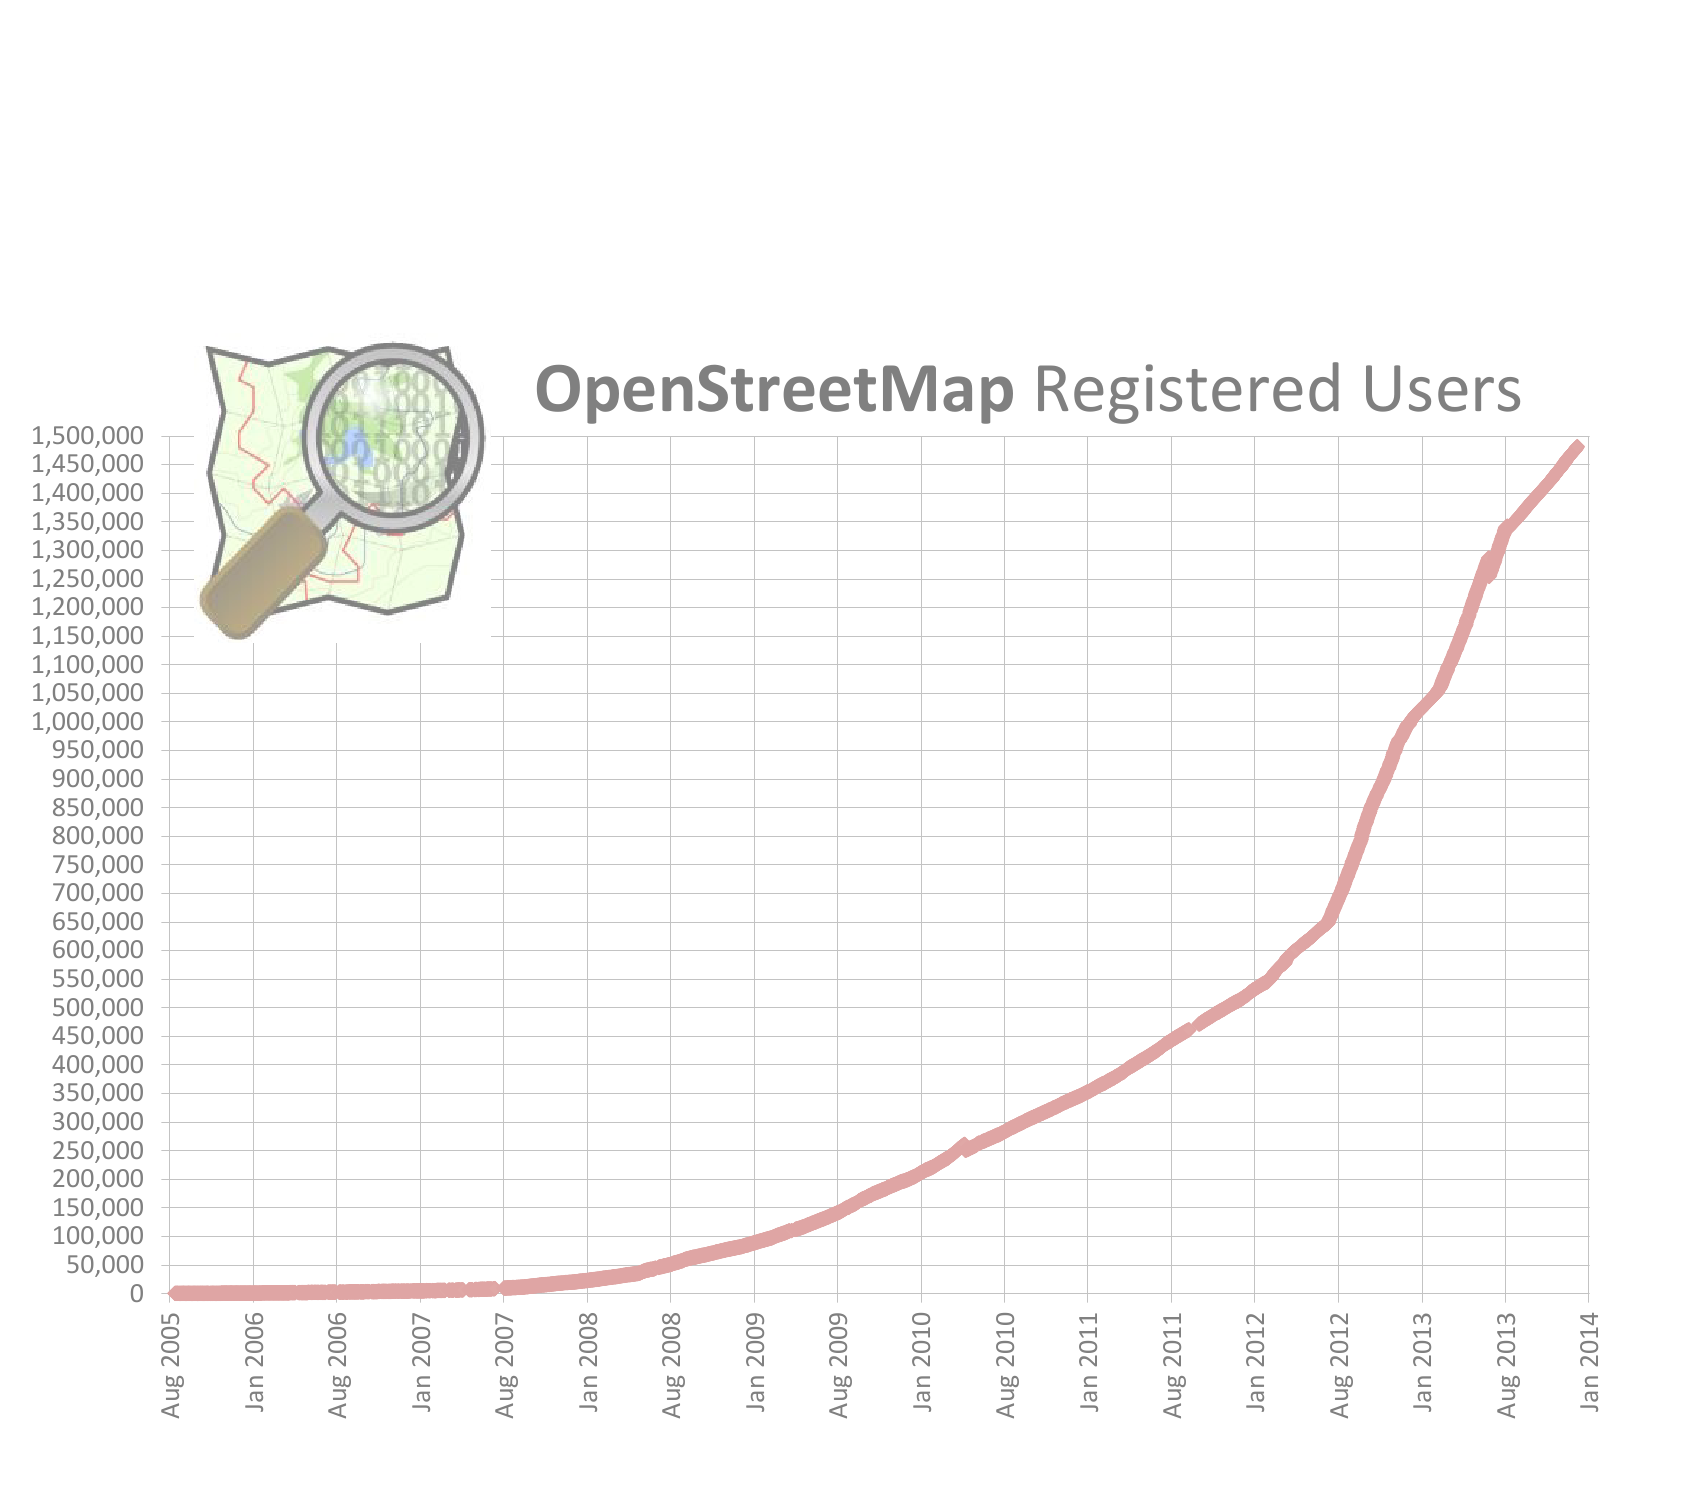
\includegraphics[height=10cm]{Osmdbstats2_users.png}}

\begin{frame}{Geschichte von OpenStreetMap}
  \vspace{0.6cm}
\begin{itemize}
  \item Start des Projekts im August 2004 durch \emph{Steve Coast}
  \item Dezember 2006 - Yahoo erlaubt abzeichnen
  \item Juli 2007 - Erste Konferenz, "`State Of The Map"'
  \item August 2007 - 10.000 Registrierte Benutzer
  \item März 2009 - 100.000 Registrierte Benutzer
  \item Januar 2010 - Haiti--Projekt
  \item November 2010 - Bing erlaubt abzeichnen
  \item Juli 2011 - Erste "`State Of The Map Europe"' in Wien
  \item Januar 2013 - 1.000.000 Registrierte Benutzer
  \item Gestern - 1.491.901 Registrierte Benutzer
\end{itemize}

\end{frame}
}




\begin{frame}{Warum OpenStreetMap?}

% wichtigster punkt: EINE geodatenbank

Wir brauchen freie Karten!

\pause
\vspace{2mm}
Vorhandene Geodaten 
\begin{itemize}
  \item	für kommerzielle Nutzung zu teuer
  \item	wenn es sie denn gibt - zB Haiti
  \item	gratis nur für Lehre und Forschung
\end{itemize}

\pause
\vspace{2mm}
Karten kommerzieller Anbieter nur sehr restriktiv nutzbar
\begin{itemize}
  \item Restriktive Lizenzen - only Free as in Beer
  \item Offline-Nutzung oft nicht erlaubt - Roaming!
  \item Absichtliche Fehler, Änderungen/Richtigstellungen?
  \pause
  \item Bsp Google TOS: Durch die Nutzung schließen sie einen rechtsgültigen Vertrag mit Google - Dürfen unmündige Personen (unter 18?) Google Maps überhaupt nutzen?
  \item Kosten! Google verlangt ab 25K API-Zugriffen/Tag!
\end{itemize}

\end{frame}

\begin{frame}{Vision einer besseren Geo-Welt}

 Sollte es nicht so sein:
  \begin{itemize}
    \item Es gibt weltweit EIN Portal für ALLE Geodaten 
    \item In einheitlichem Format (WGS84, Dezimalgrad und UTF-8)
    \item Wo man keine Anträge stellen muss, sondern einfach einen Ausschnitt wählen und Rohdaten runterladen kann
    \item Alte Versionen verfügbar (Um Änderungen zu tracken)
    \item Fehler melden kann, oder besser: gleich selbst ausbessern
    \item Alle Daten unter einen offenen Lizenz nutzen kann
  \end{itemize}

  \begin{columns}[c]
        \column{.5\textwidth}
        \begin{center}
  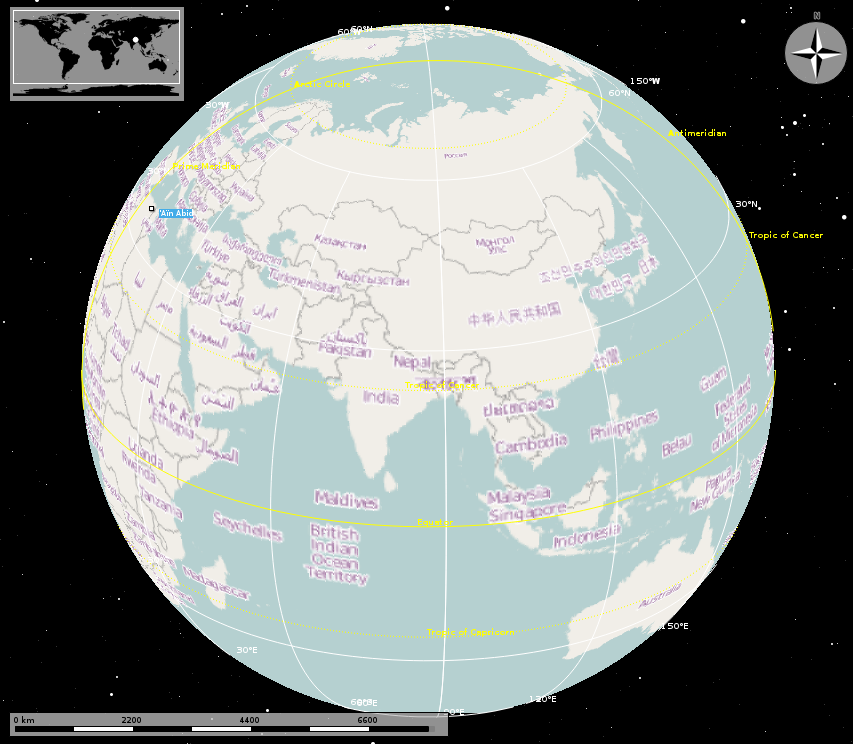
\includegraphics[width=3.5cm]{marble.png}
  \end{center}
        \column{.5\textwidth}
      \begin{center}
    
\includegraphics[width=2.5cm]{cc-by-sa.pdf}
  \end{center}
\end{columns}

\end{frame}

\section{Wie funktioniert OpenStreetMap?}

\begin{frame}{Woher kommen unsere Daten?}

\begin{itemize}
  \item Freiwillige tragen ihr Wissen bei: Jeder weis viel über seine Umgebung:
	\begin{itemize}
	  \item Hausnummern, Straßennamen,
	  \item Restaurants, Bars, POIs, ...
  \end{itemize}
  \pause
  \item Bei Mapping-Parties werden gezielt Gebiete verbessert...
\end{itemize}

 \begin{center}
 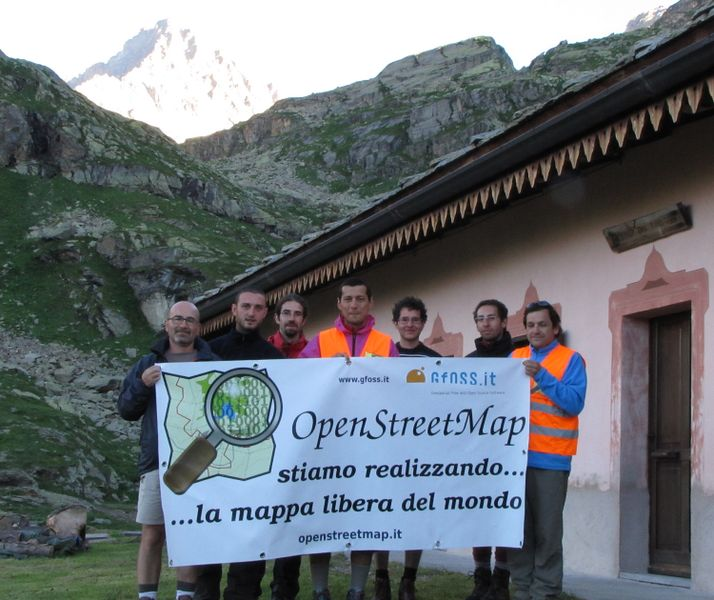
\includegraphics[width=5cm]{alps_mp.jpg}
 \end{center}

\end{frame}

\begin{frame}{Lizenz}

Die Daten stehen unter der Open Database Licence - Entspricht etwa Creative Commons - Attribution - Sharealike für Daten.
\begin{itemize}
  \item Jeder darf die Daten, auch kommerziell verwenden
  \item Quelle: "`OpenStreetMap and Contributors, ODbL"' muß angegeben werden.
\end{itemize}

 \begin{center}
 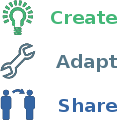
\includegraphics[width=1cm]{ODbL.png}
 \hspace{2cm}
 
\includegraphics[width=1.5cm]{cc-by-sa.png}
 \end{center}

\pause
Die Web-Karten auf \href{http://osm.org}{openstreetmap.org} sind CC-BY-SA.

\end{frame}

\section{Wie OpenStreetMap nutzen?}

\begin{frame}{Interaktive Web-Karten}

Hauptseite: \href{http://osm.org}{www.OpenStreetMap.org}

 \begin{center}
 \includegraphics[width=9cm]{mainpage.png}
 \end{center}



\end{frame}

\begin{frame}{Spezialkarten:}


  \begin{table}[htbp]
    \centering
    \begin{tabular}{r|l}
      Radkarte  &  \url{http://opencyclemap.org} \\
      Wanderkarte & \url{http://hikebikemap.de} \\
      Rauchfrei-Karte & \url{http://OpenGastroMap.org} \\
      Rollstuhl-Karte & \url{http://wheelmap.org} \\
      Seekarte & \url{http://OpenSeaMap.org} \\
\pause
      200 weitere: & siehe \href{http://wiki.openstreetmap.org/wiki/List\_of\_OSM\_based\_Services}{OSM-Wiki} \\
%      Interaktive Informationskarte & http://openstreetbrowser.org
    \end{tabular}
  \end{table}

  Blitzschnelles Routing: \url{http://osrm.at} \hspace{1cm} \includegraphics[width=2.5cm]{shoes.jpg}

\end{frame}

\begin{frame}{Mobil Nutzen}
	Apps:
 
 \begin{itemize}
   \item  Android ( \textgreater 70) \url{http://wiki.osm.org/Android}
   \item  iPhone ( \textgreater 60 )  \url{http://wiki.osm.org/Apple\_iOS}
   \item  Blackberry ( 8 ) \url{http://wiki.osm.org/BlackBerry\_OS}
 \end{itemize}
 
 \begin{center}
 \includegraphics[width=5cm]{tablet.jpg}
 \end{center}

 Natürlich auch auf Navis, am OSM-freundlichsten sind Garmin: \href{http://wiki.osm.org/Garmin}{wiki.osm.org/Garmin}!

\end{frame}

  \subsection{ OpenStreetMap Verbessern}

\begin{frame}{OpenStreetMap Verbessern}

  Eine große Auswahl an Editoren steht fürs Web, Desktop- und Mobilnutzung zur Verfügung

  \begin{itemize}
    \item Web:
    \begin{itemize}
	    \item Hauptseite - Edit: iD (JavaScript)
      \item JOSM web-start
      \item oder auch einfach nur Fehler melden!
	      \pause
    \end{itemize}
    \item Mobile (Auswahl): Alle siehe  \href{http://wiki.openstreetmap.org/wiki/Android\#OpenStreetMap\_editing\_features}{Android}, \href{http://wiki.openstreetmap.org/wiki/Apple\_iOS\#OpenStreetMap\_editing\_features}{iOS}:
    \begin{itemize}
      \item Vespucci: Ausgewachsener Editor
      \item osmaptuner: Existierende POIs ergänzen
      \item OsmTracker: GPS-Tracks, Audio, schnell POIs hinzufügen
    \end{itemize}
  \item Desktop
    \begin{itemize}
      \item \href{http://josm.openstreetmap.de}{JOSM}
      \item \href{http://merkaartor.be}{Merkaartor}
      \item ArcGIS (seit 10.1)
    \end{itemize}
  \end{itemize}

\end{frame}

\begin{frame}{Die Zukunft... 3D! }
  Neu! Jetzt auch in 3D! Beispielsweise auf \href{http://maps.osm2world.org/?zoom=17&lat=47.06156&lon=15.46983&layers=BF0FTFFF}{maps.osm2world.org}.

  \includegraphics[width=0.9\textwidth]{3d.png}


\end{frame}

\begin{frame}{Hilfe}

\begin{itemize}
  \item Fragen? OSM-Infostand am Geoday!
\end{itemize}
 \begin{center}
	  \includegraphics[width=4cm]{osm_workshop.jpg}
 \end{center}
\begin{itemize}
  \item Dokumentation: \href{http://wiki.openstreetmap.org}{wiki.openstreetmap.org}
  \item Immer noch etwas unklar? $\Rightarrow$ Mailingliste \href{http://lists.openstreetmap.org/listinfo/talk-at}{talk-at}
  \pause
  \item \href{http://wiki.openstreetmap.org/wiki/Graz/Stammtisch}{Stammtisch Graz} jedes Monat - der nächste Montag, 17.6.2013, Brot und Spiele!
\end{itemize}

\end{frame}

\section{Ende}

\begin{frame}{Vielen Dank für die Aufmerksamkeit!}

  Folien zum Ageo Forum am 16.1.2014, Wien
\vspace{1cm}

Erstellt mittels \LaTeX Beamer, Quelltext: \href{https://github.com/species/vortrag-osm-ageo}{Github}.
\vspace{1cm}

\href{mailto:michael.maier@student.tugraz.at}{Michael Maier}

Twitter: \href{https://twitter.com/osmgraz}{@osmgraz}
\vspace{1cm}

Folien unter: 
\includegraphics[width=1cm]{cc-by-sa.pdf}. 

Alle Daten ODbL, OpenStreetMap Contributors.

\end{frame}

\end{document}
